\section{Section 5.1}
\subsection{Shalev 11.2}
The ides is that searching over all the spaces of functions wihtout validation is meaningful only when we have a very small number of samples for training.
In this case, reducng the estimation error is the main goal, and therefore the main objective is to \textcolor{blue}{increase the number of samples }for training the 
models $\mathfrak{h}_i$. On the contrary, if \textcolor{blue}{we have too many examples}, then learning them individually on less data and the cross validating will reduce the modelling
error incurred by choosing only one type of model. In this case it is highly probable that the best model may not be the one with lowest training error. In orer to mitigate this
we will set aside some examples(namely, $\alpha m$) for validation. 
error

\subsection{ESL 7.10}
To be done.


\section{5.2}
\subsection{Q1}
The following table summarizes the results of both SVM and ligistic regression results with \textbf{best $C$ after cross validation}
\\
\\
\begin{tabular}{c | c | c | c | c | c }
    $Run_{number}$  & $C_{logi}$ & $Score_{logi-reg}$  & $Score_{logi-unreg}$ & $C_{svm}$ & $Score_{svm}$
     \\ \hline
    1 & 10 & 0.8412 & 0.79365 & 10 & 0.873
     \\ \hline
    2 & 10 & 0.793 & 0.714 & 10 & 0.793
     \\ \hline
    3 & 10 & 0.873 & 0.809 & 10 & 0.873
    \\ \hline
    4 & 100 & 0.773 & 0.79 & 100 & 0.873
    \\ \hline
    5 & 10 & 0.88 & 0.8412 & 10 & 0.873
    \\ \hline
\end{tabular}
\newpage
\subsection{Q2}
The following table summarizes the results for Ridge regression, however the Scikit Support vector regression model
does not work on multiple feature output, so only ridge regression results are presented with \textbf{best $\alpha$ after Cross validation}
\\
\\
\begin{tabular}{c | c | c | c  }
    $Run_{number}$  & $\alpha_{ridge}$ & $Score_{ridge-reg}$  & $Score_{linear-unreg}$ 
     \\ \hline
    1 & 10 & 0.519 & 0.389 
     \\ \hline
    2 & 10 & 0.4875 & 0.2732 
     \\ \hline
    3 & 10 & 0.5039 & 0.327
    \\ \hline
    4 & 100 & 0.5185 & 0.399
    \\ \hline
    5 & 10 & 0.546 & 0.39 
    \\ \hline
\end{tabular}

\section{Section 5.3}
\subsection{16.3 Shalev and Schwartz}
\normalfont The objective is to solve the optimization problem in the representer theorem format.
After substituting the value of $w = \alpha^TX$ the optimization problem becomes
$$
    \underset{\alpha}{min} \frac{\lambda}{2}\alpha^T G \alpha + \frac{1}{2m}\sum_{i =1}^{i=m}(\alpha^TG_i - y_i)^2
$$

Now lets take the derivative of the above equation with respect to $\alpha$ and set it to zero.
$$
    \frac{\partial}{\partial \alpha} \frac{\lambda}{2}\alpha^T G \alpha + \frac{1}{2m}\sum_{i =1}^{i=m}(\alpha^TG_i - y_i)^2 = 0
$$

$$
    {\lambda}G \alpha   +  \frac{1}{m}\sum_{i = 1}^{i=m} (\alpha^TG_i\alpha - y_i)G_i =  0
$$

On rearranging with $G_i^T \alpha = \alpha^T G_i$,
$$
    {\lambda}G \alpha  + \frac{1}{m}\sum_{i = 1}^{i=m} G_i G_i^T \alpha  =  \sum_{i = 1}^{i=m}y_i G_i
$$
Taking alpha common we get,

$$
    \alpha^* = \left( {\lambda}G  + \frac{1}{m} \sum_{i = 1}^{i = m} G_i G_i^T\right)^{-1} \sum_{i = 1}^{i=m}y_i G_i 
$$


\subsection{16.4 Shalev and Schwartz}
We will find a mapping $\psi$ that achieves this.
$$
min(x, y)  = \sum_{i = 1}^{i = N} I_{\{x \leq i\}} I_{\{y \leq i\}}
$$
The above function can be summarized using a dot product
$$
    min(x,y) = \begin{bmatrix} 1 & 1 & 1 & 1 & \ldots & 0 & 0 
    \end{bmatrix} \times \begin{bmatrix} 1 \\ 1 \\ 1\\ \\ . \\. \\ 0  \\ 0\end{bmatrix} = \psi(x)^T \psi(y)
$$
$\psi(x)$ is a vector that has a set of ones until it reaches the x'th position in the series $1 ... n$

\subsubsection{Mohri 6.1}
We know that $K(x, y) = \psi(x)^T \psi(y)$ for some $\psi : \chi \rightarrow  H$.
For the new $K'$ set $\psi(l)' = \frac{\psi(l)}{\alpha(l)}  \ \  \,\alpha(x) > 0 $
Then 
$$
K'(x, y) = \psi'(x)^T \psi'(y)
$$
\subsubsection{Mohri 6.2a}
\label{part_a}

\begin{gather}
    cos(x - y) = cosx cos y  + sinx sin y \\
                = \psi(x)^T \psi(y) + \phi(x)^T \phi(y)\\
                 = k_1(x, y) + k_2(x, y)
\end{gather}

\subsubsection{Part 6.2b}
Use the exact same technique as [\ref{part_a}]  instead of $\psi(x) = cos(x)$ let $\psi(x) = cos(x^2) $
\subsubsection{Part 6.2c}
Here let us just \textbf{Break the sum into individual terms and the product into its basic unit}
$$
    cos(x_i^2 - y_i^2) = cos(\vb{1_i}^T \vb{x}) cos(\vb{1_i}^T\vb{y}^2) + cos(\vb{1_i}^T \vb{x}) cos(\vb{1_i}^T\vb{y}^2) 
$$
The iea sis that now it has been split into $\psi_i(x) = cos(\vb{1_i}^T \vb{x})$ and $\phi(x) = sin(\vb{1_i}^T \vb{x})$
And \textcolor{green}{The sum and product of kernels remains a kernel} This completes the proof.

\subsubsection{Part 6.2d}
The idea was given as a hint to use monotonicity,
consider the function
$$
f(\theta) = \sum_{i, j} \frac{c_i c_j \theta^{x_i + x_j}}{x_1 + x_j}
$$
Note that $f(\theta) = c^TGc $ Where G is my kernel Matrix that I must show is positive semidefinite.
$$
    \frac{\partial f(\theta)}{\partial \theta} = \sum_{i, j} \frac{c_i c_j (x_i + x_j)\theta^{x_i + x_j - 1}}{x_1 + x_j} = \sum_{i, j} c_ic_ja^{x_i}a^{x_j}
$$
Now we can see that the function $f(\theta)$ is monotonic as the RHS boils down to $c^TKc$ where $k(x, y) = a^x \times a^y$ which is a kernel. 
\\
Now, since the function is monotonic, $f(1) \ge f(0) = 0$. So we get that $G \succcurlyeq 0$ Hence proved.

\subsubsection{Part 6.2e}
$$
cos \angle(x, x')  = \frac{x^Tx'}{\|x\| \|x'\|} = \psi(x)^T \psi(x')
$$
where $\psi(x) = \frac{x}{\|x\|}$
Hence proved

\subsubsection{Part 6.2f}
Lests break the exponent down
$$
    exp(-\lambda( sin(x - y)^2)) = \exp( -\lambda (1 - cos^2( x- y))) = \exp(\lambda cos^2(x - y)) \ times \exp( - \lambda)
$$
Now the second part is just a  positive constant , let us look at the first part, it is of the form
$$
    \exp(\lambda k(x)) = 1 + \lambda k(x) + \frac{\lambda^2 k(x)^2}{2!} + \frac{\lambda^3 k(x)^3}{3!} + \ldots k_n(x)
$$
We already proved that cos(x - y) is a kernel in \ref{part_a} and we know that $\lambda > 0$. This is  sufficient along with 
the \textbf{sum,product and limiting theorems} to prove that the first part is a kernel.

\subsubsection{Part 6.2h}
Using the integrals in the Hints you can see that the function is a product of the two integrals
$$
    k(x,y) = min(x, y)  - xy = x(1 - y)  \ \text{ if } x \leq y \text{ and } y(1 - x) \text{ otherwise}
$$

Now consider the Integrals 
\begin{gather}
    \int_{0}^{1} 1_{t \le x} 1_{t \le y} \ dt  = \int_{0}^{1} \psi(x)^T \psi(y) \ dt  = \  \textbf{Limiting sum of Kernels }
    \\
    I_1 = min(x, y) = x  \ or \  y
    \\
%% Now consider the greater than case
    \int_{0}^{1} 1_{t \ge x} 1_{t \ge y} \ dt  = \int_{0}^{1} \phi(x)^T \phi(y) \ dt  = \textbf{Limiting sum of Kernels }
    \\
    I_2  = 1 - max(x, y) = 1 - x  \ or  \ 1 - y
\end{gather}
We can see that the function is a product of the two integrals which are both Kernels. Hence proved.

\newpage
\subsection{Q3}
The plots are as follows
\begin{figure}[H]
    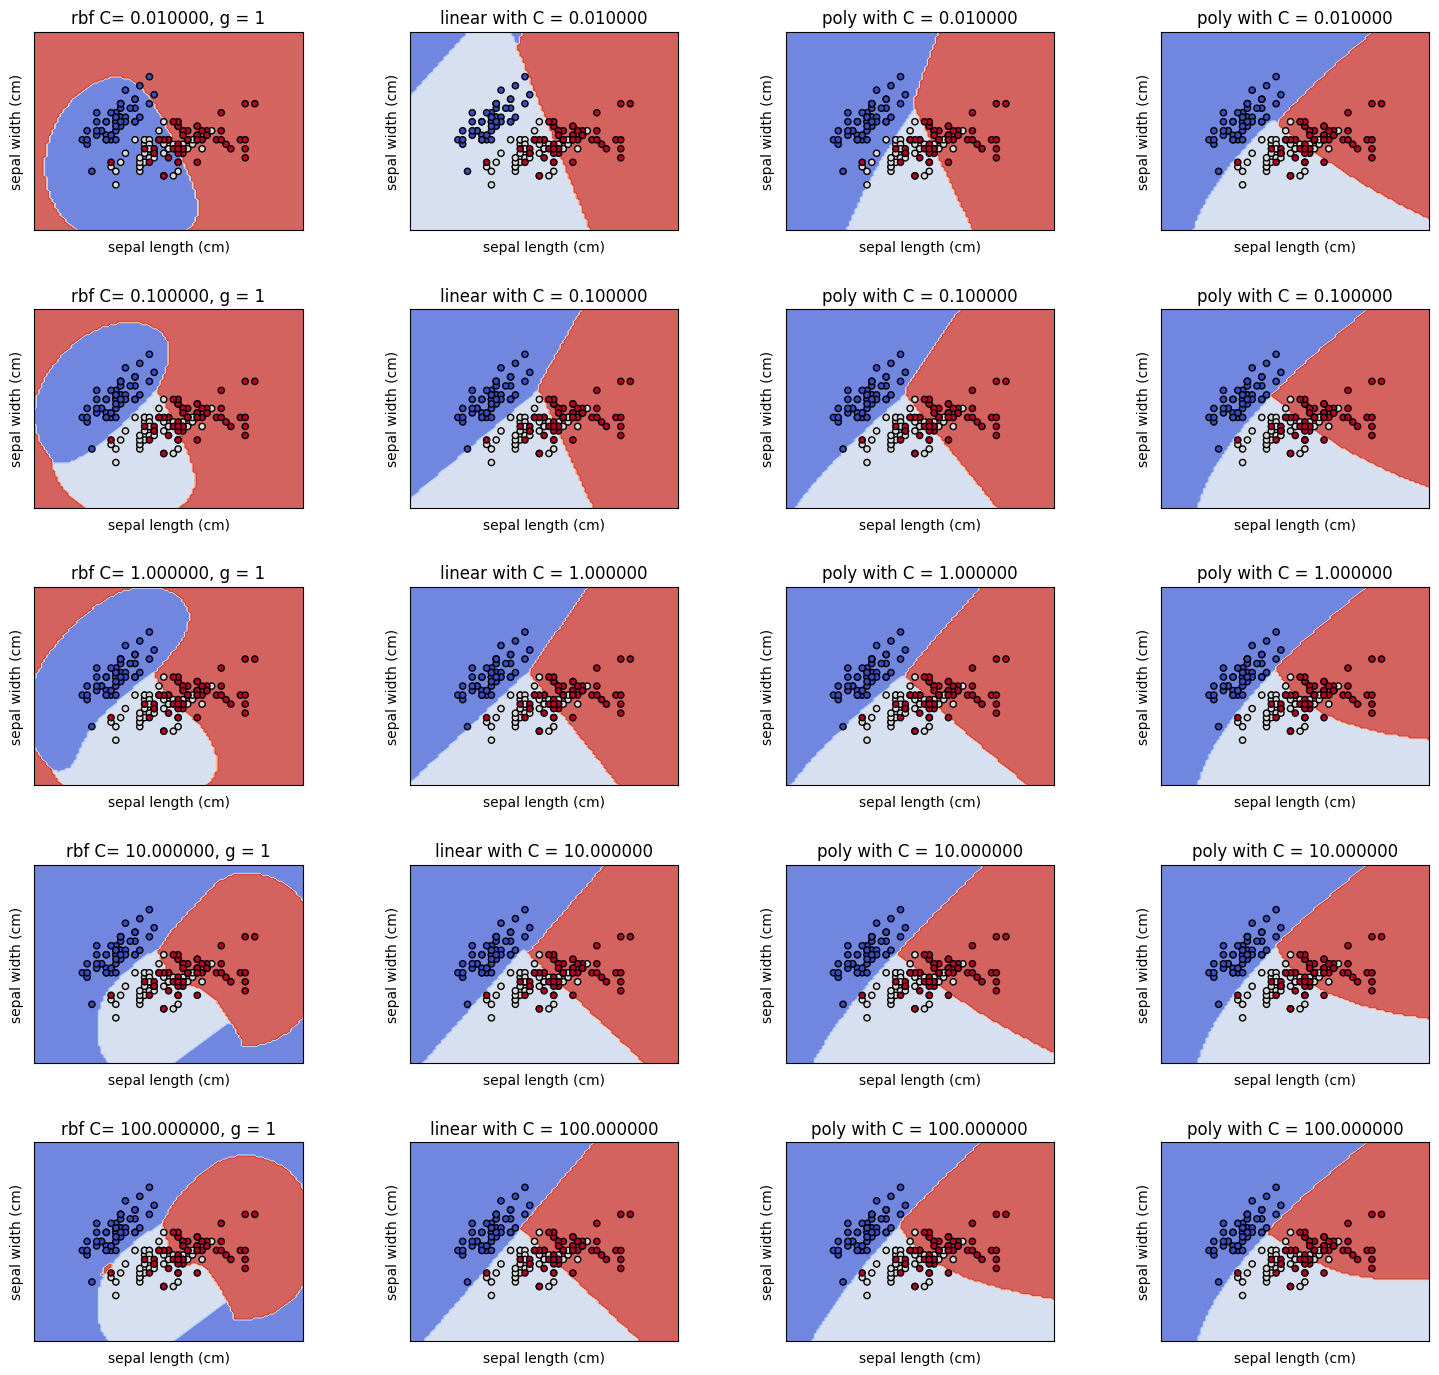
\includegraphics[scale = 0.45]{img/output.png}
    \caption{$\gamma = 1$}
    \label{fig:q3.1}
\end{figure}
\begin{figure}[H]
    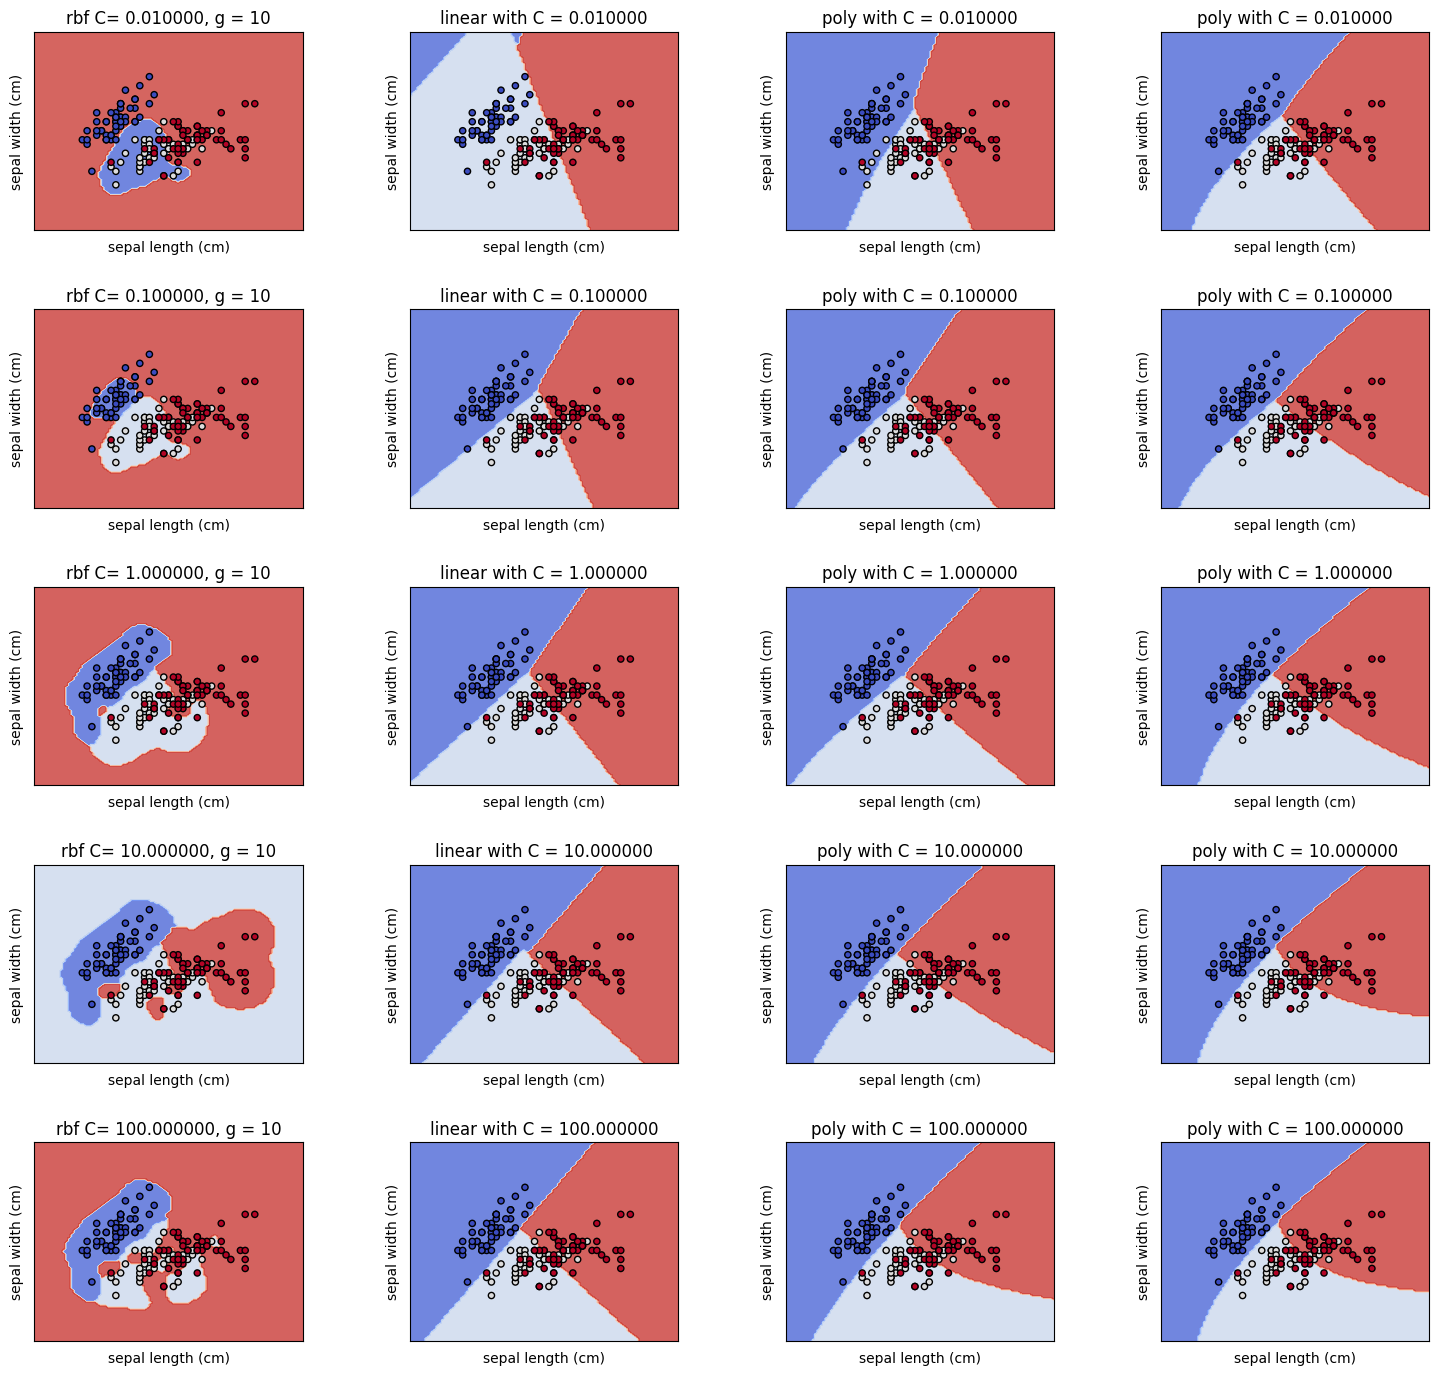
\includegraphics[scale = 0.45]{img/output2.png}
    \caption{$\gamma = 10$}
    \label{fig:q3.2}
\end{figure}
\begin{figure}[H]
    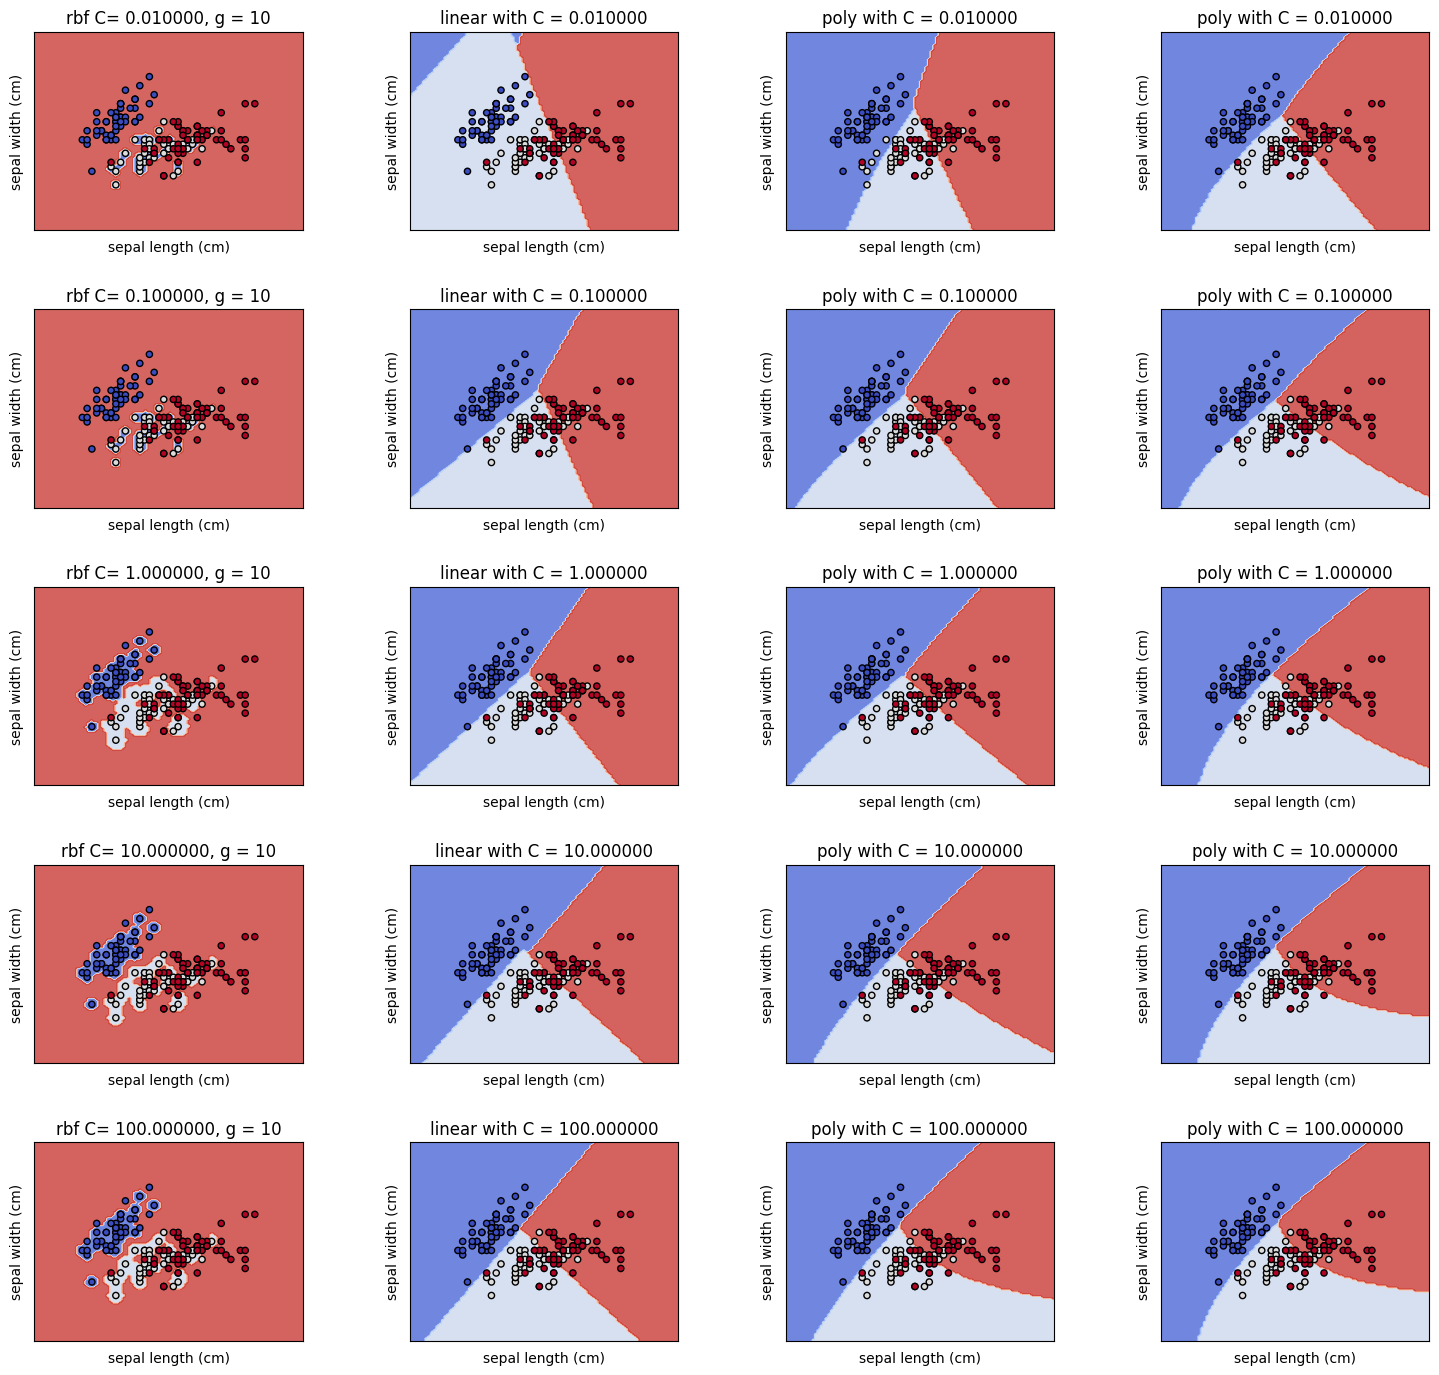
\includegraphics[scale = 0.45]{img/output3.png}
    \caption{$\gamma = 100$}
    \label{fig:q3.3}
\end{figure}
\begin{figure}[H]
    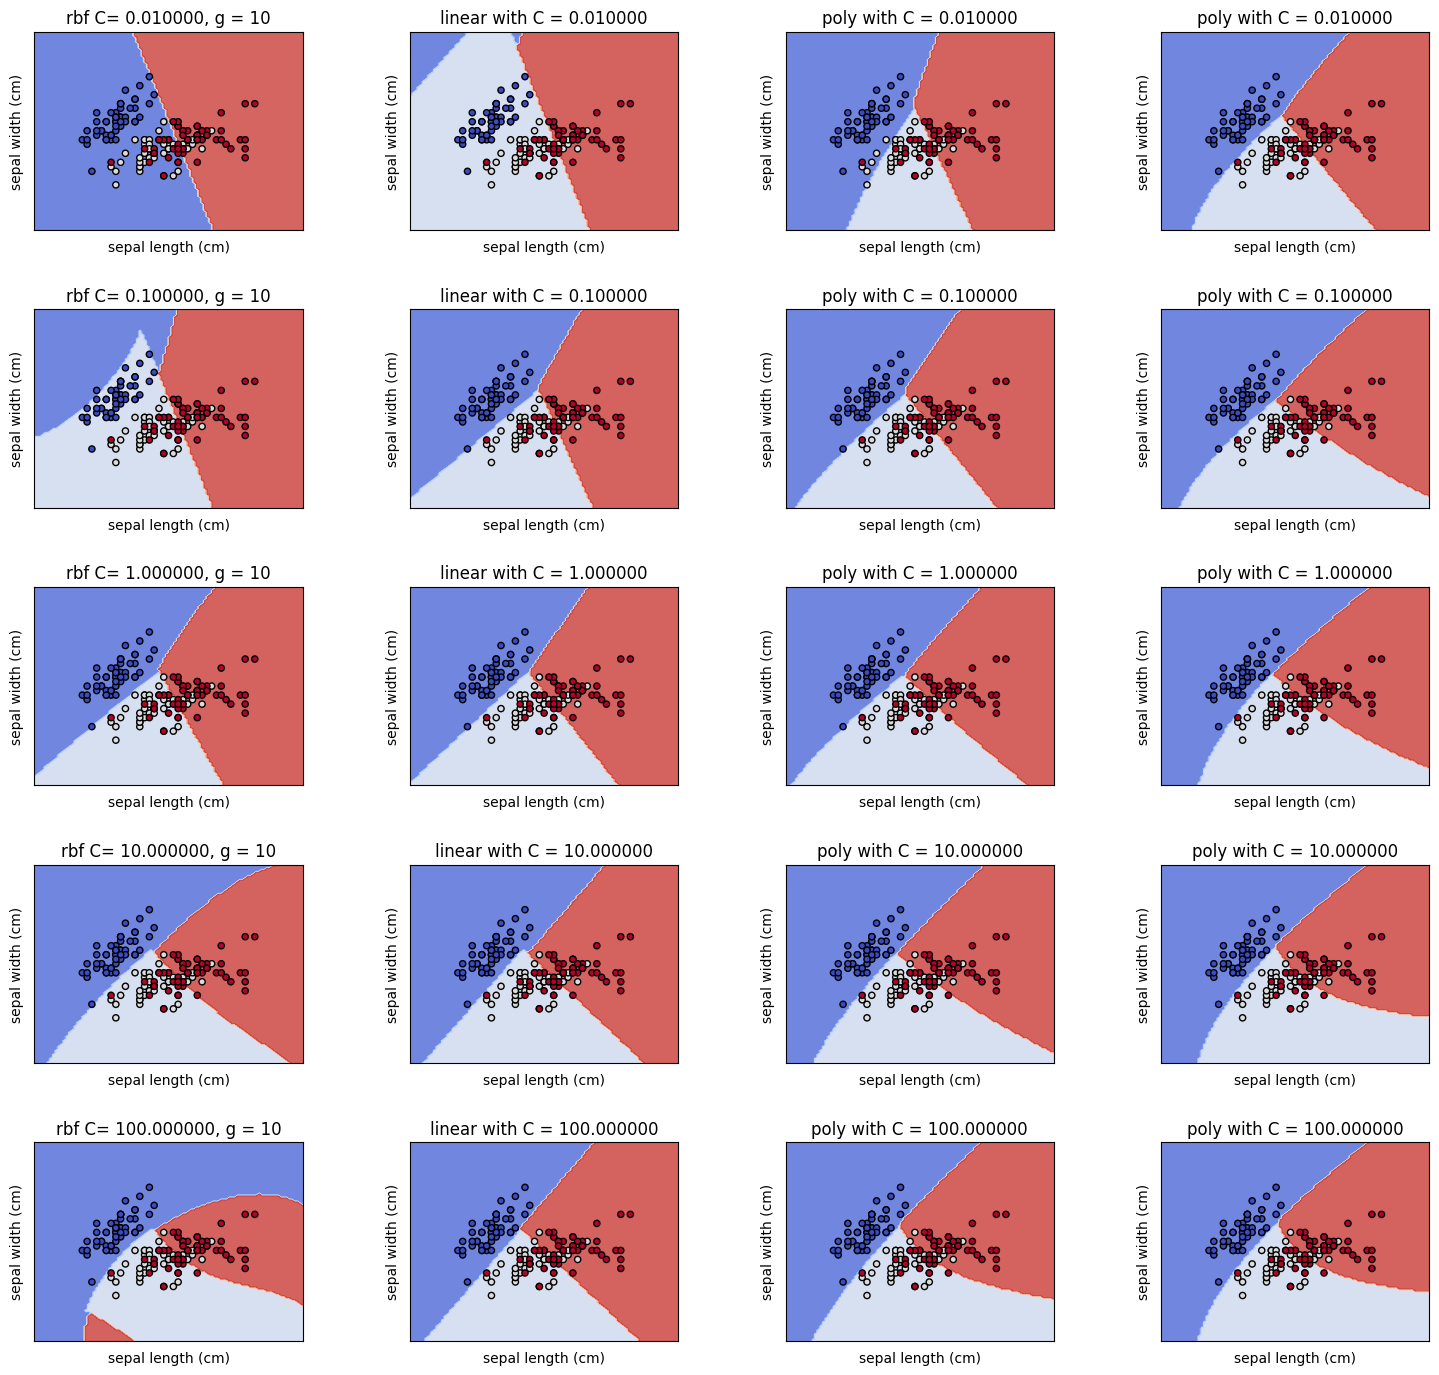
\includegraphics[scale = 0.45]{img/output4.png}
    \caption{$\gamma = 0.1$}
    \label{fig:q3.4}
\end{figure}
